 \begin{enumerate}
\item When water is filled carefully in a glass, one can fill it to a height \(h\) above the rim of the glass due to the surface tension of water. To calculate \(h\), just before water starts flowing, model the shape of the water above the rim as a disc of thickness \(h\) having semicircular edges, as shown schematically in the figure. When the pressure of water at the bottom of this disc exceeds what can be withstood due to the surface tension, the water surface breaks near the rim and water starts flowing from there. If the density of water, its surface tension and the acceleration due to gravity are \(10^3\text{ kg m}^{-3}\), \(0.07\text{ Nm}^{-1}\) and \(10\text{ ms}^{-2}\), respectively, the value of \(h\) (in mm) is \_.
\end{enumerate}

\begin{center}
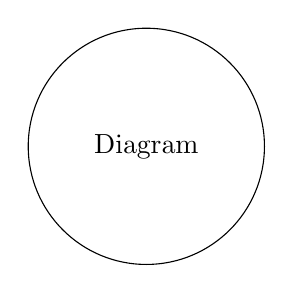
\begin{tikzpicture}
  \node [draw, circle, minimum size=3cm] (Diagram) {Diagram};
\end{tikzpicture}
\end{center}